\section{Screen Recording and Synchronization}
The actions and points of view (POV) of each participant were recorded using Open Broadcaster Software (OBS). An initial approach involved using a private network and Network Display Interface (NDI) to aggregate all screen captures onto a single device for synchronized recording. However, network bandwidth limitations caused performance issues. To address this, OBS was run locally on each machine, minimizing frame drops and network dependency. Each OBS instance was remotely triggered via a BitFocus Companion Webserver on the same network, enabling accurate synchronization for post-processing. OBS's chapter marker feature was also used to indicate the start of facial feature insertions, simplifying later reference.

\begin{figure}[H]
    \centering
    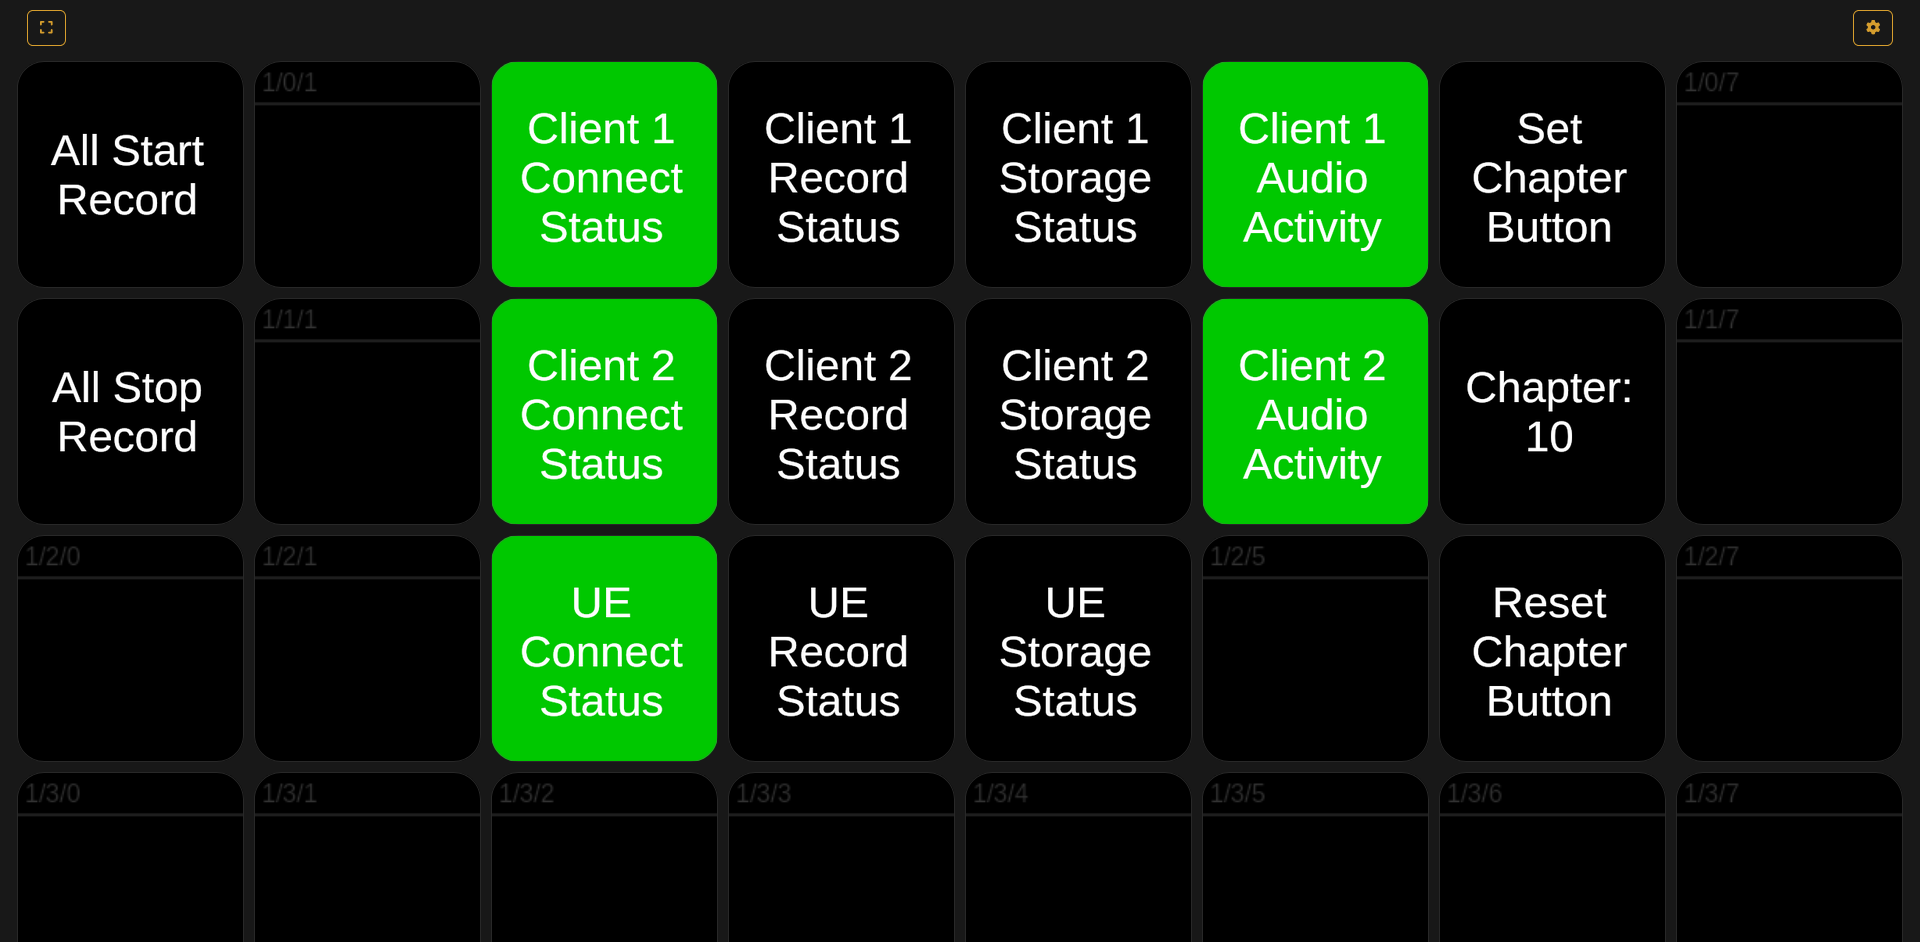
\includegraphics[width=\textwidth]{images/CompanionControl.png}
    \caption{The BitFocus Companion Webserver interface used to control OBS instances.}
    \label{fig:obs_recording}
\end{figure}

